\documentclass[12pt,border=1pt]{standalone}
\usepackage[T1]{fontenc}
\IfFileExists{newtxtext.sty}{\usepackage{newtxtext,newtxmath}}{\usepackage{mathptmx}}
\usepackage{amsmath,amssymb}
\usepackage[table]{xcolor}
\usepackage{tikz}
\usetikzlibrary{arrows.meta,positioning,fit,calc,decorations.pathreplacing}
\tikzset{blk/.style={draw=black!55,rounded corners=2pt,align=center,font=\footnotesize,inner sep=4pt,minimum height=1.05cm},
         nn/.style={blk,fill=orange!12,draw=orange!70!black},
         lat/.style={blk,fill=blue!8,draw=blue!60!black},
         io/.style={blk,fill=black!3},
         arr/.style={-{Stealth[length=2.2mm]},thick,draw=black!65}}
\definecolor{capblue}{RGB}{47,84,150}
\definecolor{linkblue}{RGB}{17,85,204}
\definecolor{ganttA}{RGB}{11,90,110}
\definecolor{ganttB}{RGB}{20,150,160}
\definecolor{rowhl}{RGB}{253,236,224}
\definecolor{rowhl2}{RGB}{224,244,238}
\begin{document}
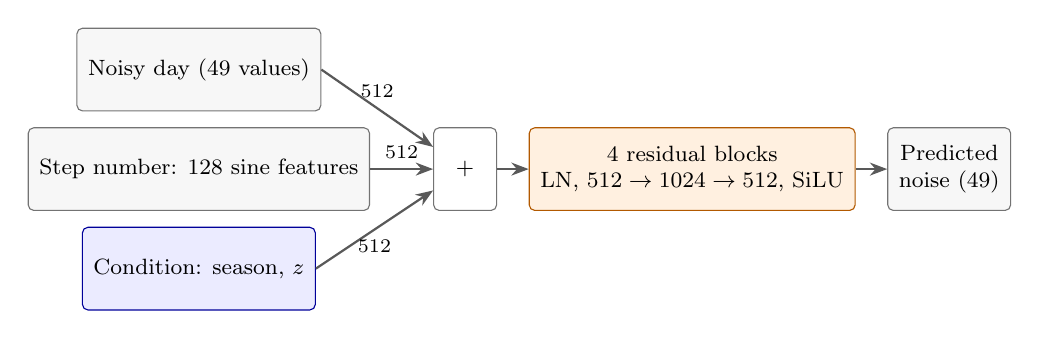
\begin{tikzpicture}[node distance=4mm]
\node[io] (x) {Noisy day (49 values)};
\node[io,below=2mm of x] (t) {Step number: 128 sine features};
\node[lat,below=2mm of t] (c) {Condition: season, $z$};
\node[blk,right=8mm of t,minimum width=8mm] (p) {$+$};
\node[nn,right=of p] (b) {4 residual blocks\\LN, $512\to1024\to512$, SiLU};
\node[io,right=of b] (o) {Predicted\\noise (49)};
\draw[arr] (x.east) -- node[above,font=\scriptsize]{512} (p);
\draw[arr] (t) -- node[above,font=\scriptsize]{512} (p);
\draw[arr] (c.east) -- node[below,font=\scriptsize]{512} (p);
\draw[arr] (p) -- (b); \draw[arr] (b) -- (o);
\end{tikzpicture}
\end{document}
